\documentclass[ignorenonframetext,]{beamer}
\setbeamertemplate{caption}[numbered]
\setbeamertemplate{caption label separator}{: }
\setbeamercolor{caption name}{fg=normal text.fg}
\beamertemplatenavigationsymbolsempty
\usepackage{lmodern}
\usepackage{amssymb,amsmath}
\usepackage{ifxetex,ifluatex}
\usepackage{fixltx2e} % provides \textsubscript
\ifnum 0\ifxetex 1\fi\ifluatex 1\fi=0 % if pdftex
  \usepackage[T1]{fontenc}
  \usepackage[utf8]{inputenc}
\else % if luatex or xelatex
  \ifxetex
    \usepackage{mathspec}
  \else
    \usepackage{fontspec}
  \fi
  \defaultfontfeatures{Ligatures=TeX,Scale=MatchLowercase}
\fi
\usetheme[]{Berlin}
% use upquote if available, for straight quotes in verbatim environments
\IfFileExists{upquote.sty}{\usepackage{upquote}}{}
% use microtype if available
\IfFileExists{microtype.sty}{%
\usepackage{microtype}
\UseMicrotypeSet[protrusion]{basicmath} % disable protrusion for tt fonts
}{}
\newif\ifbibliography
\hypersetup{
            pdftitle={Planification de maintenances des aéronefs militaires},
            pdfborder={0 0 0},
            breaklinks=true}
\urlstyle{same}  % don't use monospace font for urls
\usepackage{longtable,booktabs}
\usepackage{caption}
% These lines are needed to make table captions work with longtable:
\makeatletter
\def\fnum@table{\tablename~\thetable}
\makeatother

% Prevent slide breaks in the middle of a paragraph:
\widowpenalties 1 10000
\raggedbottom

\AtBeginPart{
  \let\insertpartnumber\relax
  \let\partname\relax
  \frame{\partpage}
}
\AtBeginSection{
  \ifbibliography
  \else
    \let\insertsectionnumber\relax
    \let\sectionname\relax
    \frame{\sectionpage}
  \fi
}
\AtBeginSubsection{
  \let\insertsubsectionnumber\relax
  \let\subsectionname\relax
  \frame{\subsectionpage}
}

\setlength{\parindent}{0pt}
\setlength{\parskip}{6pt plus 2pt minus 1pt}
\setlength{\emergencystretch}{3em}  % prevent overfull lines
\providecommand{\tightlist}{%
  \setlength{\itemsep}{0pt}\setlength{\parskip}{0pt}}
\setcounter{secnumdepth}{0}

\title{Planification de maintenances des aéronefs militaires}
\author{Franco Peschiera, Alain Haït, Olga Battaïa}
\institute{ISAE SUPAERO}
\date{June 06, 2018}

\begin{document}
\frame{\titlepage}

\begin{frame}
\tableofcontents[hideallsubsections]
\end{frame}

\section{Introduction}\label{introduction}

\begin{frame}{Planification Thèse}

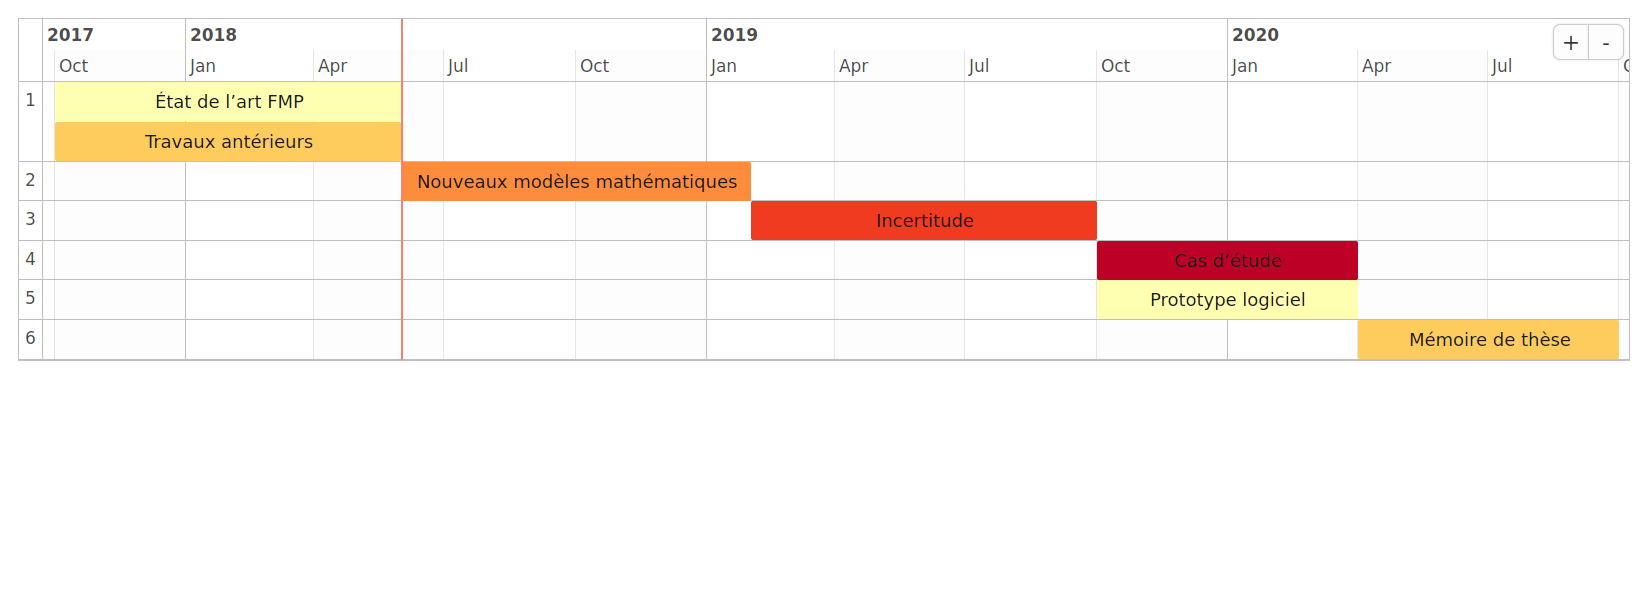
\includegraphics[width=1\linewidth]{./../../img/gantt_thesis}

\end{frame}

\section{Problème}\label{probleme}

\begin{frame}{Avions}

Une flotte hétérogène d'avions, dont chacun a les caractéristiques
suivantes :

\begin{itemize}[<+->]
\tightlist
\item
  Butée calendrier.
\item
  Butée horaire.
\item
  Fonctionnalités.
\end{itemize}

\end{frame}

\begin{frame}{Missions}

Un ensemble de missions à réaliser, chacune avec :

\begin{itemize}[<+->]
\tightlist
\item
  Dates de début et fin.
\item
  Un nombre nécessaire d'avions par mois.
\item
  Une consommation d'heures par avion et par mois.
\item
  Des fonctionnalités requises.
\end{itemize}

\end{frame}

\begin{frame}{Maintenances}

Chaque maintenance suit les règles suivantes :

\begin{itemize}[<+->]
\tightlist
\item
  La \emph{durée est de 6 mois} consécutifs.
\item
  Le nombre maximal d'heures de vol entre deux maintenances est
  \emph{1000h}.
\item
  Le nombre maximal de mois entre deux maintenances est \emph{60 mois}.
\end{itemize}

\end{frame}

\begin{frame}{États possibles}

En résumé, voici les états logiques possibles d'un aéronef :

\begin{itemize}[<+->]
\tightlist
\item
  En mission.
\item
  En maintenance.
\item
  En stockage.
\item
  Disponible.
\end{itemize}

\end{frame}

\begin{frame}{Objectifs}

\begin{itemize}[<+->]
\tightlist
\item
  Maximiser la disponibilité.
\item
  Minimiser le coût (en réduisant le nombre de maintenances).
\end{itemize}

\end{frame}

\begin{frame}{Problème (exemple)}

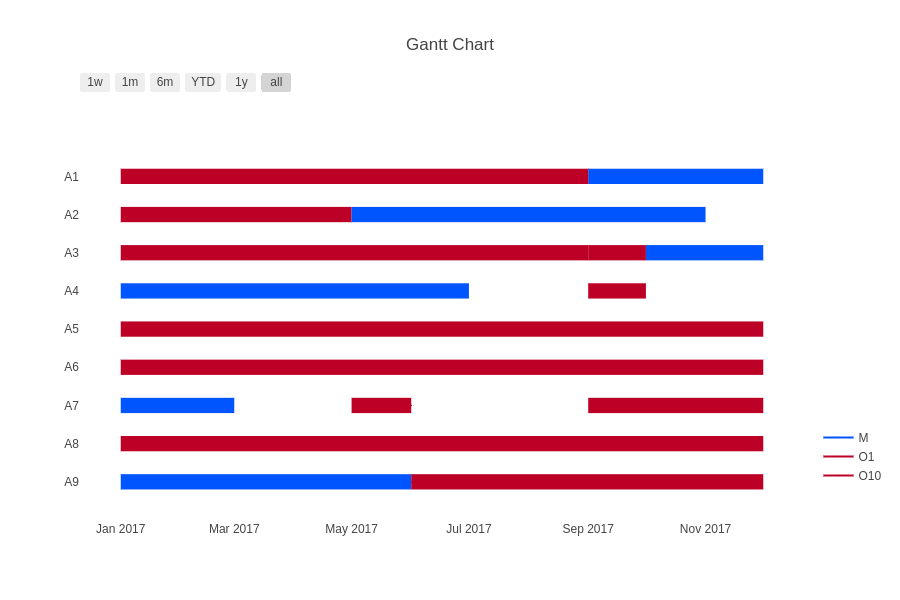
\includegraphics[width=1\linewidth]{./../../img/calendar}

\end{frame}

\begin{frame}{Contraintes / Règles / Objectifs}

\begin{itemize}[<+->]
\tightlist
\item
  RQ001: heures de missions.
\item
  RQ002: aéronefs affectés.
\item
  RQ003: besoins de maintenance.
\item
  RQ004: durée de maintenance.
\item
  RQ005: disponibilité.
\item
  RQ006: capacité de maintenance.
\item
  RQ007: état final.
\item
  RQ008: stockage.
\end{itemize}

\end{frame}

\section{État de l'art}\label{etat-de-lart}

\begin{frame}{État de l'art (1)}

\begin{quote}
FMP: Flight and Maintenance Planning problem.
\end{quote}

\begin{itemize}[<+->]
\tightlist
\item
  Minimisation du nombre maximal de maintenances. Affectations
  quotidiennes. États-Unis, Cho (2011).
\item
  Maximisation de disponibilité de vol.~Affectations mensuelles Grèce,
  Kozanidis (2008).
\item
  Minimisation du nombre maximal de maintenances. Affectations
  mensuelles. Pays-Bas. Verhoeff, Verhagen, and Curran (2015).
\end{itemize}

\end{frame}

\begin{frame}{État de l'art (2)}

Les travaux précédents:

\begin{itemize}[<+->]
\tightlist
\item
  ont étudié de flottes homogènes: nous avons une flotte hétérogène.
\item
  n'ont ni le mêmes contraintes ni les mêmes objectifs.
\item
  n'affectent pas les avions aux missions.
\end{itemize}

\end{frame}

\section{Modèle}\label{modele}

\begin{frame}{Modèle: fonction objectif}

\begin{align}
    & \text{Min}\; W_1 m_{max} + W_2 u_{max}
\end{align}

\pause

Minimiser le nombre maximal de maintenances et le nombre maximal de
non-disponibilités.

\begin{align}
    &\sum_{t' \in \mathcal{T}^{s}_t} \sum_{i \in \mathcal{I}} m_{it'} + N_t \leq m_{max}
    &t \in \mathcal{T} \\
    &\sum_{t' \in \mathcal{T}^{s}_t} \sum_{i \in \mathcal{I}} m_{it'} + N_t + D_t\leq u_{max}
    &t \in \mathcal{T}
\end{align}

\end{frame}

\begin{frame}{Modèle: contraintes principales}

Besoins des missions et incompatibilités entre les missions et les
maintenances.

\begin{align}
&\sum_{i \in \mathcal{I}_j} a_{jti} = R_j
&j \in \mathcal{J}, t \in \mathcal{T}_j\\
&\sum_{t' \in \mathcal{T}^{s}_t} m_{it'} + \sum_{j \in \mathcal{J}_t \cap \mathcal{O}_i} a_{jti} \leq 1
& t \in \mathcal{T}, i \in \mathcal{I}
\end{align}

\end{frame}

\begin{frame}{Modèle: contraintes de flux}

Calcul des heures de vol restantes pour chaque avion:

\begin{align}
& rut_{it} \leq rut_{it-1} + H m_{it} - \sum_{j \in \mathcal{J}_t \cap \mathcal{O}_i} a_{jti} H_j & t =1, ..., \mathcal{T}, i \in \mathcal{I}\\
& rut_{i0} = Rut^{Init}_i
        & i \in \mathcal{I}\\
& rut_{it} \geq H m_{it}
        & t \in \mathcal{T}, i \in \mathcal{I}\\
& rut_{it} \in [0,H]
        & t \in \mathcal{T}, i \in \mathcal{I} \\
& \sum_{i \in \mathcal{I}} rut_{it} \geq Rut^{Init}_{sum}
        & t = |\mathcal{T}|
\end{align}

\end{frame}

\section{Résultats}\label{resultats}

\begin{frame}{Expériences}

Des instances ont déjà été testées:

\begin{longtable}[]{@{}lllllll@{}}
\toprule
id & \(\|\mathcal{J}\|\) & \(\|\mathcal{T}\|\) & assign & objective &
time (s) & bound\tabularnewline
\midrule
\endhead
I\_0 & 9 & 11 & 310 & 62.0 & 0.7 & 62.0\tabularnewline
I\_1 & 9 & 21 & 650 & 63.0 & 68.7 & 63.0\tabularnewline
I\_2 & 9 & 31 & 990 & 63.0 & 3600.1 & 62.0\tabularnewline
I\_3 & 9 & 41 & 1249 & 64.0 & 3603.9 & 61.7\tabularnewline
I\_4 & 10 & 11 & 530 & 82.0 & 0.9 & 82.0\tabularnewline
I\_5 & 10 & 21 & 1070 & 83.0 & 144.0 & 83.0\tabularnewline
I\_6 & 10 & 31 & 1610 & 83.0 & 3600.1 & 82.0\tabularnewline
I\_7 & 10 & 41 & 2069 & 84.0 & 3609.1 & 81.8\tabularnewline
I\_8 & 11 & 11 & 1080 & 139.0 & 530.6 & 139.0\tabularnewline
I\_9 & 11 & 21 & 2120 & 149.0 & 3600.0 & 139.9\tabularnewline
\bottomrule
\end{longtable}

\end{frame}

\section{Perspectives}\label{perspectives}

\begin{frame}{Perspectives}

\begin{itemize}[<+->]
\tightlist
\item
  \textbf{L'amélioration du modèle mathématique}: casser les symétries,
  reformuler les objectifs.
\item
  \textbf{Solutions techniques alternatives}: essayer d'autres méthodes
  de résolution.
\item
  \textbf{Continuer le dialogue avec les utilisateurs}: ajouter de
  nouvelles contraintes, valider les résultats.
\end{itemize}

\end{frame}

\section{Références}\label{references}

\begin{frame}{Références / Questions?}

\hypertarget{refs}{}
\hypertarget{ref-Cho2011}{}
Cho, P. 2011. ``Optimal Scheduling of Fighter Aircraft Maintenance.''
PhD thesis, Massachusetts Institute of Technology.

\hypertarget{ref-Kozanidis2008}{}
Kozanidis, G. 2008. ``A Multiobjective Model for Maximizing Fleet
Availability under the Presence of Flight and Maintenance
Requirements.'' \emph{Journal of Advanced Transportation} 43 (2):
155--82.

\hypertarget{ref-Verhoeff2015}{}
Verhoeff, M., W. J C Verhagen, and R. Curran. 2015. ``Maximizing
operational readiness in military aviation by optimizing flight and
maintenance planning.'' \emph{Transportation Research Procedia} 10
(July). Elsevier B.V.: 941--50.
doi:\href{https://doi.org/10.1016/j.trpro.2015.09.048}{10.1016/j.trpro.2015.09.048}.

\end{frame}

\end{document}
